
%=======================   Default Templete   ==================
\documentclass[a4paper]{article}
% \documentclass[12pt]{extreport}
\usepackage{graphicx}

% file with some default definations
%%%%%%%%%%%%%%%%%%%%%%%%%%%%%%%%%%%%%%%%%
% Lachaise Assignment
% Structure Specification File
% Version 1.0 (26/6/2018)
%
% This template originates from:
% http://www.LaTeXTemplates.com
%
% Authors:
% Marion Lachaise & François Févotte
% Vel (vel@LaTeXTemplates.com)
%
% License:
% CC BY-NC-SA 3.0 (http://creativecommons.org/licenses/by-nc-sa/3.0/)
% 
%%%%%%%%%%%%%%%%%%%%%%%%%%%%%%%%%%%%%%%%%

%----------------------------------------------------------------------------------------
%	PACKAGES AND OTHER DOCUMENT CONFIGURATIONS
%----------------------------------------------------------------------------------------

\usepackage{amsmath,amsfonts,stmaryrd,amssymb} % Math packages

\usepackage{enumerate} % Custom item numbers for enumerations

\usepackage[ruled]{algorithm2e} % Algorithms

\usepackage[framemethod=tikz]{mdframed} % Allows defining custom boxed/framed environments

\usepackage{listings} % File listings, with syntax highlighting
\lstset{
	basicstyle=\ttfamily, % Typeset listings in monospace font
}

%----------------------------------------------------------------------------------------
%	DOCUMENT MARGINS
%----------------------------------------------------------------------------------------

\usepackage{geometry} % Required for adjusting page dimensions and margins

\geometry{
	paper=a4paper, % Paper size, change to letterpaper for US letter size
	top=2.5cm, % Top margin
	bottom=3cm, % Bottom margin
	left=3.5cm, % Left margin
	right=3.5cm, % Right margin
	headheight=14pt, % Header height
	footskip=1.5cm, % Space from the bottom margin to the baseline of the footer
	headsep=1.2cm, % Space from the top margin to the baseline of the header
	%showframe, % Uncomment to show how the type block is set on the page
}

%----------------------------------------------------------------------------------------
%	FONTS
%----------------------------------------------------------------------------------------

\usepackage[utf8]{inputenc} % Required for inputting international characters
\usepackage[T1]{fontenc} % Output font encoding for international characters

\usepackage{XCharter} % Use the XCharter fonts

%----------------------------------------------------------------------------------------
%	COMMAND LINE ENVIRONMENT
%----------------------------------------------------------------------------------------

% Usage:
% \begin{commandline}
%	\begin{verbatim}
%		$ ls
%		
%		Applications	Desktop	...
%	\end{verbatim}
% \end{commandline}

\mdfdefinestyle{commandline}{
	leftmargin=10pt,
	rightmargin=10pt,
	innerleftmargin=15pt,
	middlelinecolor=black!50!white,
	middlelinewidth=2pt,
	frametitlerule=false,
	backgroundcolor=black!5!white,
	frametitle={Command Line},
	frametitlefont={\normalfont\sffamily\color{white}\hspace{-1em}},
	frametitlebackgroundcolor=black!50!white,
	nobreak,
}

% Define a custom environment for command-line snapshots
\newenvironment{commandline}{
	\medskip
	\begin{mdframed}[style=commandline]
}{
	\end{mdframed}
	\medskip
}

%----------------------------------------------------------------------------------------
%	FILE CONTENTS ENVIRONMENT
%----------------------------------------------------------------------------------------

% Usage:
% \begin{file}[optional filename, defaults to "File"]
%	File contents, for example, with a listings environment
% \end{file}

\mdfdefinestyle{file}{
	innertopmargin=1.6\baselineskip,
	innerbottommargin=0.8\baselineskip,
	topline=false, bottomline=false,
	leftline=false, rightline=false,
	leftmargin=2cm,
	rightmargin=2cm,
	singleextra={%
		\draw[fill=black!10!white](P)++(0,-1.2em)rectangle(P-|O);
		\node[anchor=north west]
		at(P-|O){\ttfamily\mdfilename};
		%
		\def\l{3em}
		\draw(O-|P)++(-\l,0)--++(\l,\l)--(P)--(P-|O)--(O)--cycle;
		\draw(O-|P)++(-\l,0)--++(0,\l)--++(\l,0);
	},
	nobreak,
}

% Define a custom environment for file contents
\newenvironment{file}[1][File]{ % Set the default filename to "File"
	\medskip
	\newcommand{\mdfilename}{#1}
	\begin{mdframed}[style=file]
}{
	\end{mdframed}
	\medskip
}

%----------------------------------------------------------------------------------------
%	NUMBERED QUESTIONS ENVIRONMENT
%----------------------------------------------------------------------------------------

% Usage:
% \begin{question}[optional title]
%	Question contents
% \end{question}

\mdfdefinestyle{question}{
	innertopmargin=1.2\baselineskip,
	innerbottommargin=0.8\baselineskip,
	roundcorner=5pt,
	nobreak,
	singleextra={%
		\draw(P-|O)node[xshift=1em,anchor=west,fill=white,draw,rounded corners=5pt]{%
		Question \theQuestion\questionTitle};
	},
}

\newcounter{Question} % Stores the current question number that gets iterated with each new question

% Define a custom environment for numbered questions
\newenvironment{question}[1][\unskip]{
	\bigskip
	\stepcounter{Question}
	\newcommand{\questionTitle}{~#1}
	\begin{mdframed}[style=question]
}{
	\end{mdframed}
	\medskip
}

%----------------------------------------------------------------------------------------
%	WARNING TEXT ENVIRONMENT
%----------------------------------------------------------------------------------------

% Usage:
% \begin{warn}[optional title, defaults to "Warning:"]
%	Contents
% \end{warn}

\mdfdefinestyle{warning}{
	topline=false, bottomline=false,
	leftline=false, rightline=false,
	nobreak,
	singleextra={%
		\draw(P-|O)++(-0.5em,0)node(tmp1){};
		\draw(P-|O)++(0.5em,0)node(tmp2){};
		\fill[black,rotate around={45:(P-|O)}](tmp1)rectangle(tmp2);
		\node at(P-|O){\color{white}\scriptsize\bf !};
		\draw[very thick](P-|O)++(0,-1em)--(O);%--(O-|P);
	}
}

% Define a custom environment for warning text
\newenvironment{warn}[1][Warning:]{ % Set the default warning to "Warning:"
	\medskip
	\begin{mdframed}[style=warning]
		\noindent{\textbf{#1}}
}{
	\end{mdframed}
}

%----------------------------------------------------------------------------------------
%	INFORMATION ENVIRONMENT
%----------------------------------------------------------------------------------------

% Usage:
% \begin{info}[optional title, defaults to "Info:"]
% 	contents
% 	\end{info}

\mdfdefinestyle{info}{%
	topline=false, bottomline=false,
	leftline=false, rightline=false,
	nobreak,
	singleextra={%
		\fill[black](P-|O)circle[radius=0.4em];
		\node at(P-|O){\color{white}\scriptsize\bf i};
		\draw[very thick](P-|O)++(0,-0.8em)--(O);%--(O-|P);
	}
}

% Define a custom environment for information
\newenvironment{info}[1][Info:]{ % Set the default title to "Info:"
	\medskip
	\begin{mdframed}[style=info]
		\noindent{\textbf{#1}}
}{
	\end{mdframed}
}

\usepackage{listings}
\lstset{language=Python, basicstyle=\normalsize\sffamily\linespread{0.8}, numbers=left, numberstyle=\small, stepnumber=1, numbersep=5pt}
\usepackage{fancyhdr}
\usepackage{pdfpages} 
\setlength{\parindent}{0pt}

\pagestyle{fancy}
\fancyhf{}
\lhead{\textbf{\NAME}}
\chead{\textbf{Course Project Report}}
\rhead{\COURSE}

\usepackage{calrsfs}
\DeclareMathAlphabet{\pazocal}{OMS}{zplm}{m}{n}
\newcommand{\La}{\mathcal{L}}
\newcommand{\Lb}{\pazocal{L}}
\newcommand{\Tb}{\pazocal{T}}

%==================Header details======================
\newcommand\NAME{Bayesian Meta Learning}
\newcommand\ANDREWID{}
\newcommand\HWNUM{4}
\newcommand\COURSE{CS771}
%======================================================
\begin{document}

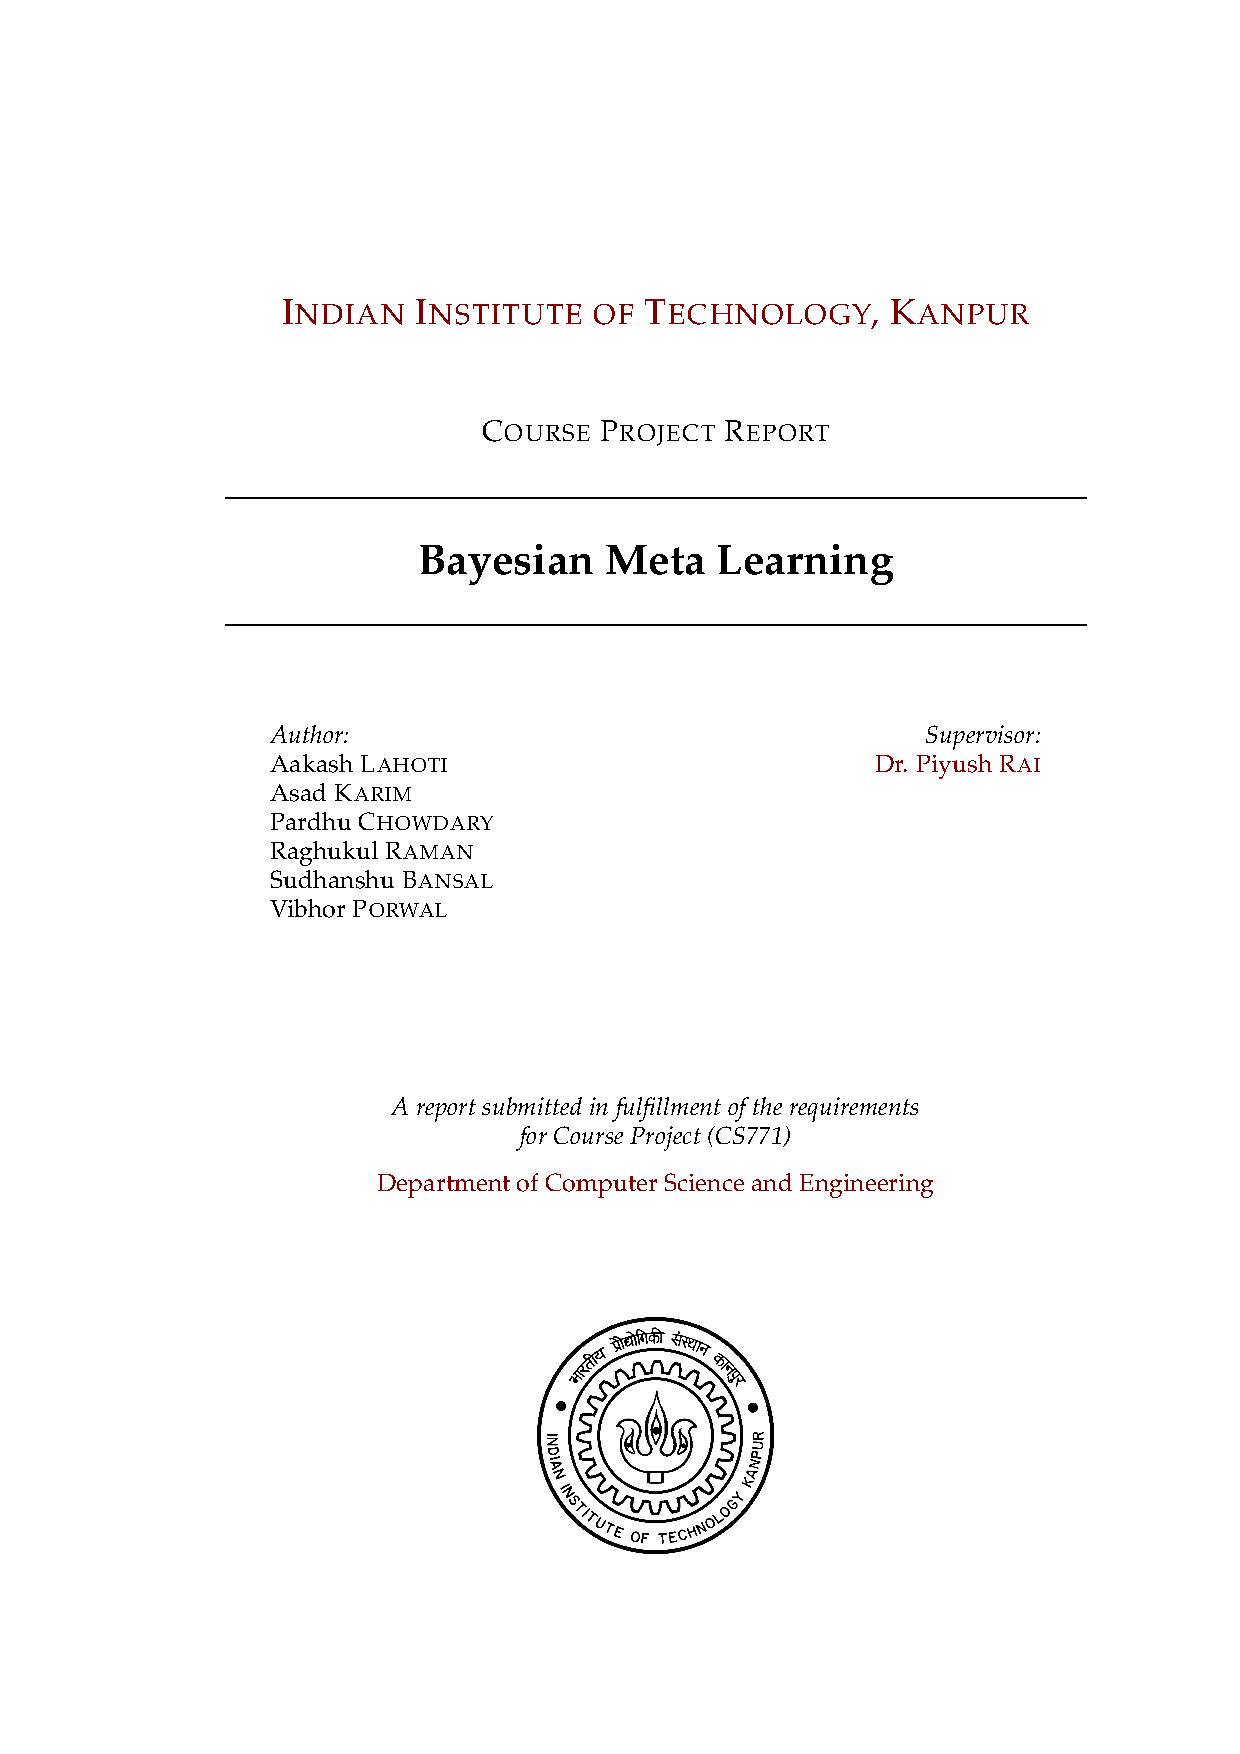
\includepdf[page={1}]{first_page.pdf}

\section{Abstract}

Machine learning algorithms generally require a lot of data to perform significantly well on any task.In contrast humans have this inherent ability to learn any task with limited experience.For example even a kid can recognize an object by looking at it only once.This is possible due to abilities such as shape bias. We will present a machine learning algorithm which tries to accomplish this task.

This domain of machine learning is known as meta-learning.The word "Meta" is used to indicate some concept about a concept . So meta-learning is basically learning about learning.Our goal is to train a model that has the ability to learn a new task with little amount of training.We will show that our approach works well on variety of supervised learning problems such as sinusoidal curve fitting(regression) and classification of hand written letters on omniglot dataset. 


\subsection*{Subsection (if any) Name}

....

\section{Literature Review}

MAML has been designed to enable fast adaptation to unseen tasks by training on statistically related tasks. The algorithm is Model-Agnostic which means that it can be used on any model trained through gradient-descent.

\subsection{Problem Formulation}
The paper presents a generic formulation applicable to tasks like regression, classification and reinforcement learning. Let $f$ denote the common model for all tasks with $\theta$ being the central parameter to be learned. It maps input $x$ to output $a$. Each Task is denoted by $$\Tb: \{{L}({x_1}, {a_1}, ... , {x_H}, {a_H}),q({x_1}),q({x_{t+1}}|{x_t,a_t}),H\}$$

here L is the task specific loss function, $q(x_1)$ is the distribution of inputs, $q(x_{t+1} |x_t,a_t )$ is the transition probability for all states , and episode length is H. \\
H is specifically for non-iid data, for example the unfolding of reinforcement learning training sample. For the supervised iid classification and regression experiments, H=1.

\subsection{Algorithm}
$p(\Tb)$ is the distribution over tasks over which we would train and test the meta-learning model. We will follow a K-Shot learning setting. First, a batch of tasks is sampled from $p(\Tb)$ and for each sample task $\Tb_i$, \textit{K} inputs are sampled from $q_i$. These sampled inputs are used to learn task specific $\theta_i$s which were initialized to the central parameter $\theta$. Then, we sample \textit{K} more inputs to evaluate that particular task with the $\theta_i$s. The sum of the loss incurred in all the tasks is used as the meta-loss function to find the optimal $\theta$. 

\begin{algorithm}[H]
	\SetAlgoLined
	\KwIn{$p(\Tb):$ Distribution over tasks, $\alpha, \beta:$ Step size hyper parameters}
	\KwOut{Parameters for this model} 
	randomly initialize $\theta$ \\ 
	\While{not done} {
		Sample batch of tasks $\Tb_i \approx p(\Tb)$ \\ 
		\For{all $\Tb_i$} {
			Sample $K$ data points $D = \{ x^{(j)}, y^{(j)}\}$ from $\Tb_i$ \\  
			Compute $\nabla_\theta \Lb_{\Tb_i}(f_\theta)$ using \textit{K} samples \\ 
			Compute adapted parameters with gradient descent: \\ 
			$\theta^{'}_{i} = \theta - \alpha\nabla_\theta \Lb_{\Tb_i}(f_\theta)$ \\ 
			Sample data points $D^{'}_i = \{ x^{(j)}, y^{(j)}\}$ from $\Tb_i$ for the meta update \\ 
		}
		Update $\theta \leftarrow \theta - \beta \nabla_\theta \sum_{\Tb_i \approx p(\Tb)} \Lb_{\Tb_i} (f_(\theta^{'}_i))$ using each $D^{'}_i$ and $\Lb_{\Tb_i}$. 
	}	
	\Return{$\theta$}
\end{algorithm}

Formally, for each $\Tb_i$, we calculate $\theta_i'$ using the \textit{K} samples by the following gradient descent update.
$$ \theta_i' = \theta - \alpha \nabla_\theta \Lb_{\Tb_i}(f_\theta) $$
Here $\alpha$ is the step size and is a hyperparameter for the model. The meta objective is minimizing the sum of loss incurred in testing the sampled tasks against $D_i$s.
$$ \min_\theta \sum_{\Tb_i \sim p(\Tb)}\Lb_{\Tb_i}(f_{\theta_i'}) = \sum_{\Tb_i \sim p(\Tb) }\Lb_{\Tb_i}(f_{\theta - \alpha \nabla_\theta \Lb_{\Tb_i}(f_\theta)}) $$
Finally, we perform the meta optimization step using gradient descent for the central parameter $\theta$ on the loss function defined above. 
$$\theta \leftarrow \theta - \beta \nabla_\theta \sum_{\Tb_i \sim p(\Tb)} \Lb_{\Tb_i} (f_{\theta^{'}_i})$$

\subsection{Algorithm for supervised learning (Regression and classification)}
To formalize in the context of meta learning, the loss function used for regression is the mean squared error loss as shown below
$$ \Lb_{\Tb_{i}}(f_\phi) = \sum_{x^{(j)}, y^{(j) }\sim\Tb_{i}} || f_{\phi}(x^{(j)}) - y^{(j)} ||^2_2 $$
where $\phi$ is the model parameter.
For classification, the loss function is given as
$$ \Lb_{\Tb_{i}}(f_\phi) = \sum_{x^{(j)}, y^{(j) }\sim\Tb_{i}} y^{(j)} \log f_{\phi}(x^{(j)}) + (1-y^{(j)}) \log (1 - f_{\phi}(x^{(j)})) $$


\subsection*{Algorithm Review}

....

\subsection*{Bayesian ML}

....

\subsection*{Reinforcement Learning}

....

\pagebreak
\section{Experiments}
Most of the experiments carried out required automated differentiation through gradient update, 
for which we used TensorFlow. 
A signification computation was required in finding the second derivative, 
in the meta gradient update step, 
which involved backpropogating the meta-gradient through gradient calculation in meta gradient objective ($\theta \leftarrow \theta - \beta \nabla_\theta \sum_{T_i \approx p(T)} L_{T_i}(f_{\theta^{'}_i}) $). \\ \\
We have tested the MAML algorithm for Regression and Classfication problem. Now let's discuss each of these experiment in details.

\subsection{Regression}
\subsubsection{Data Set}
We tested our model on the task of regressing from the input to output of a sine wave,
where each task had a different amplitude and phase, where amplitude varies within $[0.1, 5.0]$ and phase varies within $[0, \pi]$. 
Note that input and output in our problem are just $1$ dimensional. 
Datapoints are sampled uniformly from $[-5.0, 5.0]$ and the loss function is simply the mean sqaured error between prediction and the ground truth.

\subsubsection{Architecture}
Our regressor is a neural network model which has $2$ hidden layers of $40$ hidden units, and each each containing activation function as ReLU. \\
While training hyperparameter $\alpha = 0.01$, and our meta optimizer is Adam \cite{adam}. 

\subsubsection{Experiment Protocol}
We performed $K$ shot learning for $K = 5, 10, 20$.

\subsubsection{Results}
\textbf{Results for $K = 5$}
\begin{table}[h!]
\centering
\begin{tabular}{c c c}
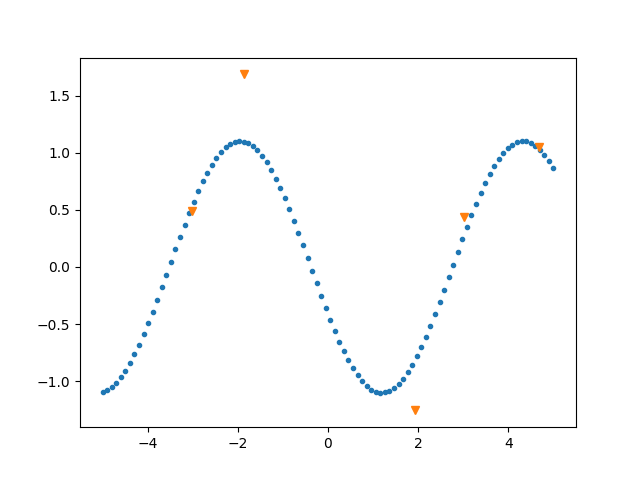
\includegraphics[width=5cm]{5shot1_1.png} & 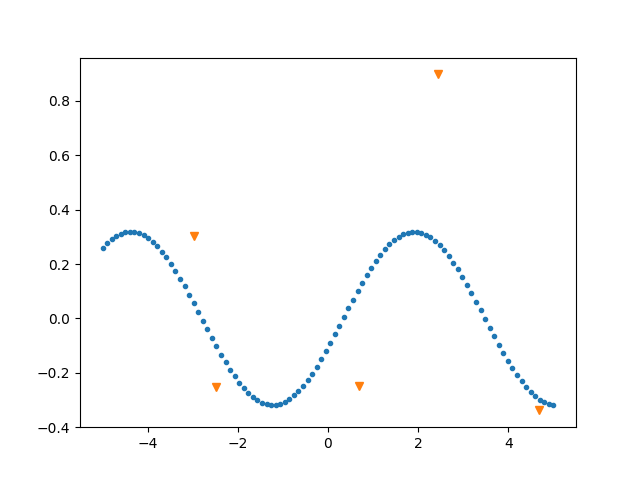
\includegraphics[width=5cm]{5shot1_2.png} & 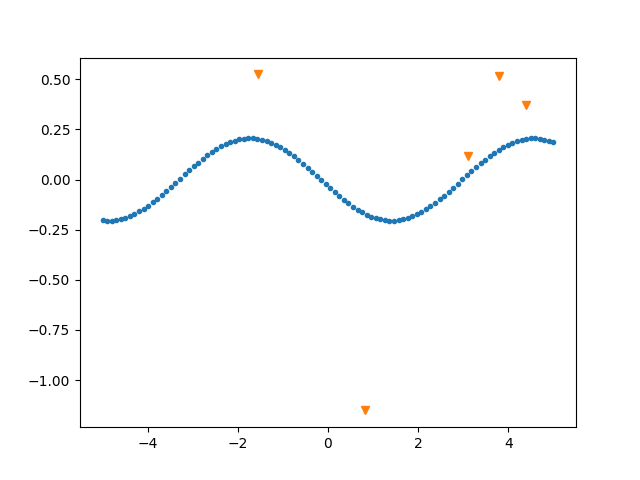
\includegraphics[width=5cm]{5shot1_3.png} \\
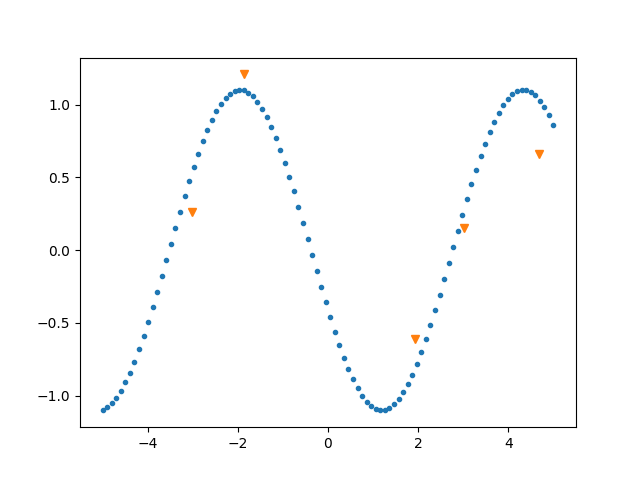
\includegraphics[width=5cm]{5shot5_1.png} & 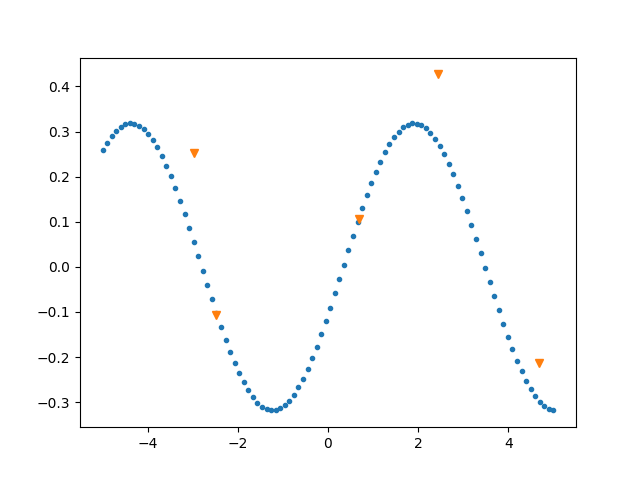
\includegraphics[width=5cm]{5shot5_2.png} & 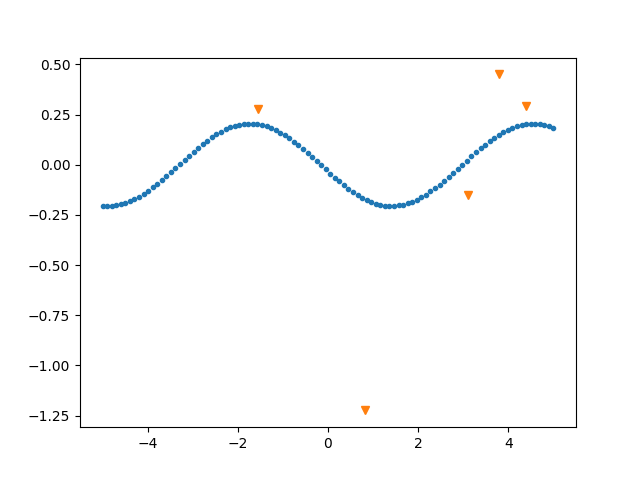
\includegraphics[width=5cm]{5shot5_3.png} \\
\end{tabular}
\end{table}

\pagebreak
\textbf{Results for $K = 10$}
\begin{table}[h!]
\centering
\begin{tabular}{c c c}
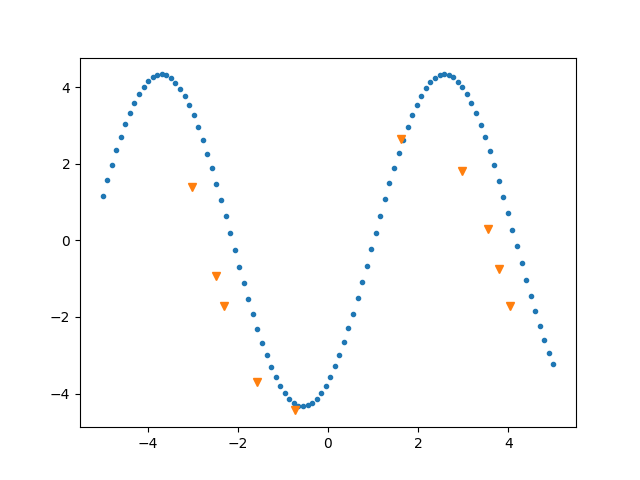
\includegraphics[width=5cm]{10shot1_1.png} & 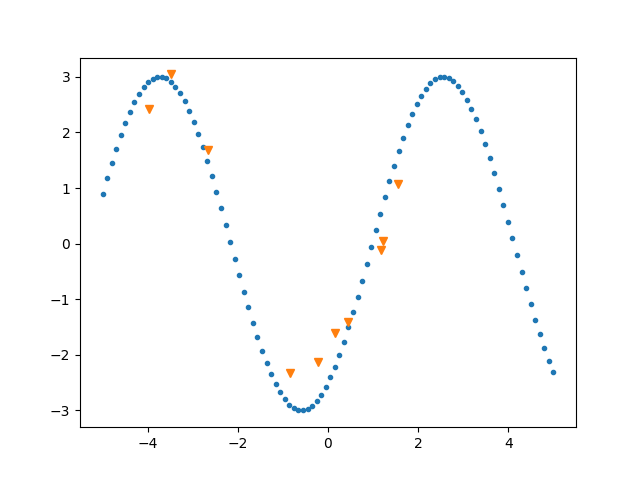
\includegraphics[width=5cm]{10shot1_2.png} & 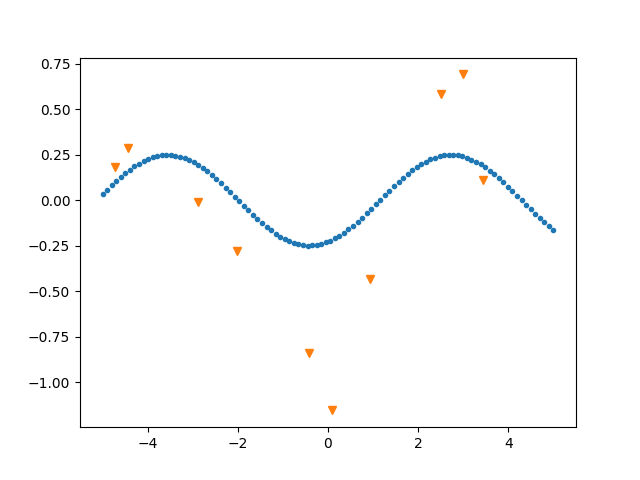
\includegraphics[width=5cm]{10shot1_3.png} \\
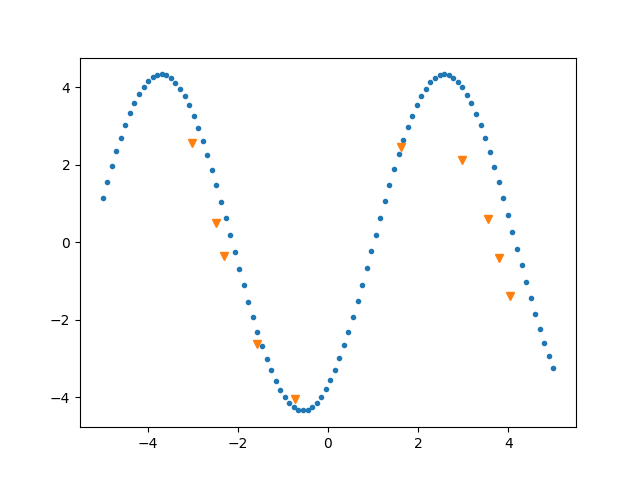
\includegraphics[width=5cm]{10shot5_1.png} & 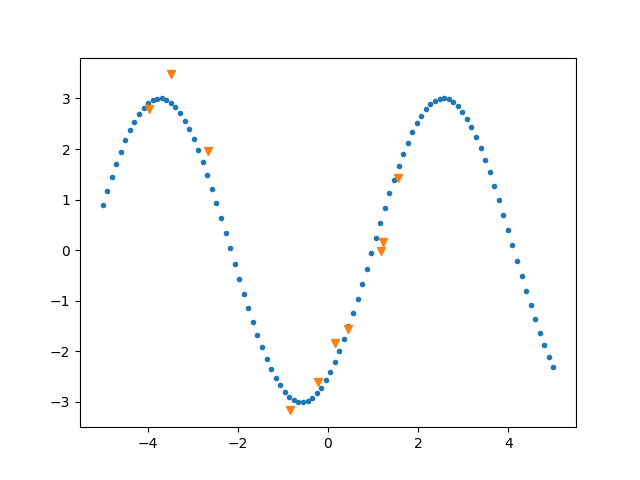
\includegraphics[width=5cm]{10shot5_2.png} & 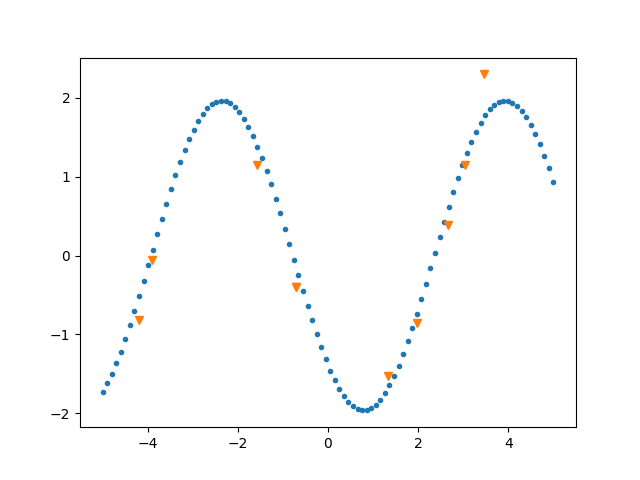
\includegraphics[width=5cm]{10shot5_3.png} \\
\end{tabular}
\end{table}
\begin{center}
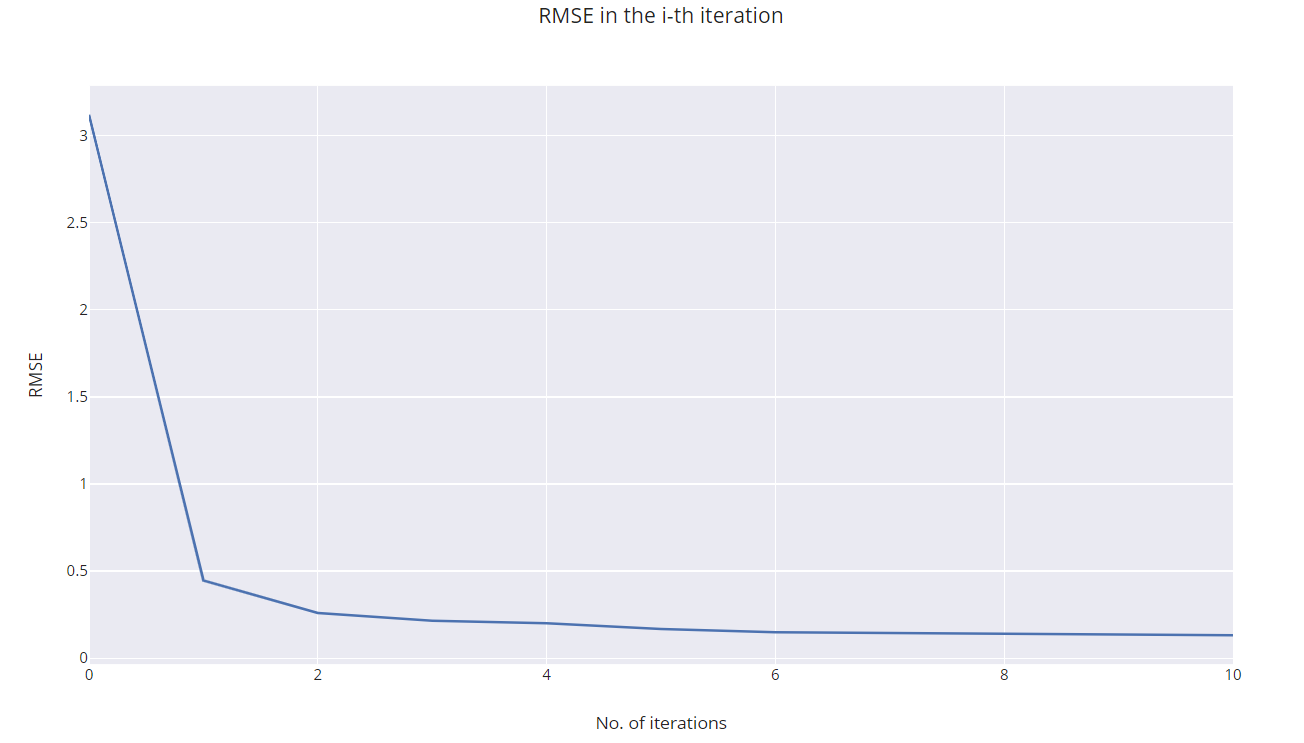
\includegraphics[width=13cm]{capture.png}
\end{center}

\subsection{Classification}
\subsubsection{Data Set}
\subsubsection{Architecture}
\subsubsection{Experiment Protocol}
\subsubsection{Results}

....

\section{Conclusion}

We found that the MAML performs reasonably well on sinusoidal curve fitting and also on the ominiglot dataset .So from this we infer that it is a pretty good method for gradient based models.So we can use it for various other problems also. 
\section{Future Work}

The model provided in the paper is simple as it works on any gradient based model.One of the possibilities could be to generalize the model we studied  to other variety of problem.We tested this method using neural networks. It would be great if we could try the method on other type of gradient based models like Kernelised ridge regression, SVMs etc. We could make multitasking initialization a standard step in reinforcement learning and deep learning.\\
Currently the method does not scale appreciably on reinforcement learning problems.So we should focus on this area also.

\subsection*{Subsection (if any) Name}

....

\section*{Future Work}

....

\subsection*{Subsection (if any) Name}

....

\subsubsection*{Acknowledgments}

....
\pagebreak
\begin{thebibliography}{9}
\bibitem{maml}
Chelsea Finn, Pieter Abbeel and Sergey Levine.
\textit{Model-Agnostic Meta-Learning for Fast Adaptation of Deep Networks.}
2017.

\bibitem{bayesian}
Taesup Kim, Jaesik Yoon, Ousmane Dia1, Sungwoong Kim, Yoshua Bengio and Sungjin Ahn.
\textit{Bayesian Model-Agnostic Meta-Learning.}
Jun 2018.

\bibitem{gradient_based}
Erin Grant, Chelsea Finn, Sergey Levine, Trevor Darrell, Thomas Griffiths.
\textit{Recasting Gradient-based Meta-Learning as hierarchical Bayes.}
Jan 2018.

\bibitem{adam}
Maclaurin, Dougal, Duvenaud, David, and Adams, Ryan.
\textit{Gradient-based hyperparameter optimization through reversible learning.}
In International Conference on Machine Learning (ICML), 2015.
\end{thebibliography}

\end{document}
